\documentclass[12pt,a4paper]{article}
% \usepackage[UTF8]{ctex}
% \usepackage{minted}
\usepackage{fontspec}
\usepackage{titletoc}
\usepackage{xeCJK}
\usepackage{graphicx}
\usepackage{amsmath}
\usepackage{indentfirst} % 中文首段缩进
\usepackage{minted} % 代码块高亮渲染

% \setmainfont[Path=/usr/share/fonts/wenquanyi/wqy-microhei/]{wqy-microhei.ttc}
% \setCJKmainfont[Path=/usr/share/fonts/wenquanyi/wqy-microhei/]{wqy-microhei.ttc}
\setmainfont[Path=/usr/share/fonts/TTF/]{DroidSansFallbackFull.ttf} % DroidSansFallbackFull.ttf Legacy
\setCJKmainfont[Path=/usr/share/fonts/TTF/]{DroidSansFallbackFull.ttf}

\graphicspath{ {img/} }

\usepackage{xcolor}
\usepackage{hyperref}
\hypersetup{
    colorlinks=true,
    linkcolor=blue,
    urlcolor=red,
    linktoc=all
}
\definecolor{bg}{rgb}{0.95,0.95,0.95}
\newcommand{\incode}[1]{\mintinline[bgcolor=bg]{c}{#1}} % 定义行内代码渲染命令
\newcommand{\codefile}[1]{\inputminted[bgcolor=bg,linenos,tabsize=4]{verilog}{code/#1}} % 定义行内代码渲染命令
	
\renewcommand{\baselinestretch}{1.1} % 定义行间距
\parindent 24pt % 重新定义缩进长度
 
%%%%%%%%%%%%%%%%%%%%%%%%%%%%%%%%%%%%%%%%%%%%%%%%%%%%%%%%%%%%%%%%
%  lengths
%    下面的命令重定义页面边距,使其符合中文刊物习惯。
%%%%%%%%%%%%%%%%%%%%%%%%%%%%%%%%%%%%%%%%%%%%%%%%%%%%%%%%%%%%%%%%
\addtolength{\topmargin}{-54pt}
\setlength{\oddsidemargin}{-0.9cm}  % 3.17cm - 1 inch
\setlength{\evensidemargin}{\oddsidemargin}
\setlength{\textwidth}{17.00cm}
\setlength{\textheight}{25.50cm}    % 24.62

\title{实验四~流水线MIPS~CPU~Cache}
\author{张海斌\thanks{学号 17307130118}}
\begin{document}
\date{2019年5月}

\maketitle

\renewcommand\contentsname{目~录}
\tableofcontents

\section{概要}

实验四添加Cache模块充当MIPS~CPU和内存之间数据通信的中介,目的是了解Cache的基本原理和构造,以及程序如何对时间、空间的局部性进行优化。Cache采用的是四路组相联高速缓存,Cache包括四个组,每个组包含四个块,每个块包含四个字的数据。块替换策略使用LRU算法。由于同时有指令内存和数据内存,所以我总共使用了两个完全相同的独立的Cache作为CPU与内存数据交流的中介。对于CPU的控制,当缓存没有命中的时候,CPU会处于暂停的状态,这个暂停状态我通过控制CPU的时钟延迟上升沿的到来来控制。

\section{功能展示}

与之前的流水线处理器相比,七段数码管的显示和开关的控制几乎是完全相同的,提供了当前Fetch阶段PC和下一个周期PC的显示和当前正在读取的机器码的显示,以及通用寄存器和数据内存数据的显示控制。只有显示内存数据需要的内存地址位数增加了一位。而LED则显示了一些更多的内容:LED[15]同样是显示处理器的时钟信号,LED[14]显示的是两个Cache是否都已就绪,LED[13]表示CPU实际接收的时钟信号(Cache未就绪时时钟上升沿信号会被屏蔽掉),LED[12]和LED[11]分别表示指令内存和数据内存对应的缓存是否命中,LED[10:7]和LED[6:3]分别显示指令内存和数据内存对应的缓存控制器中有限状态机的状态值。

\section{代码结构}

\begin{figure}[htbp]
	\centering
	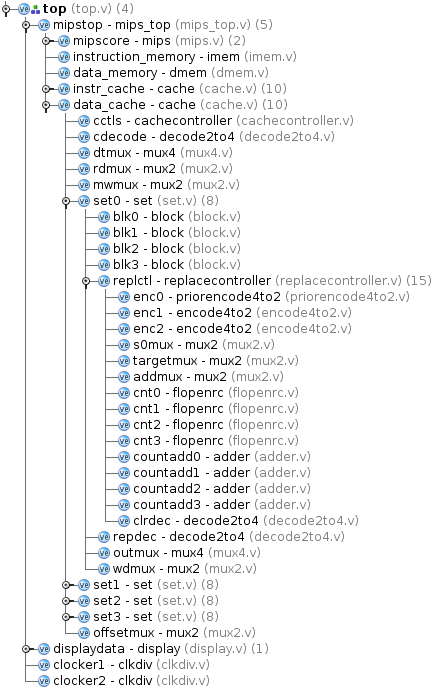
\includegraphics[width=0.5\textwidth]{cache-struct}
	\caption{Cache模块层次结构图}
	\label{fig:struct}
\end{figure}

Figure \ref{fig:struct} 展现了MIPS的结构和\incode{Cache}模块中的各个具体模块结构。总体上来说,MIPS的结构没有太大的变化,只在\incode{mips_top}模块内增加了两个\incode{cache}模块。\incode{cache}模块的组成主要有两个部份:Cache控制器\incode{cachecontroller}模块和四个完全相同的组\incode{set}模块。在每个组\incode{set}模块下,又包含了块\incode{block}模块和块替换策略控制模块\incode{replacecontroller}。

\section{模块设计}

\subsection{\incode{block}缓存块}

\begin{listing}[h]
	\definecolor{bg}{rgb}{0.95,0.95,0.95}
	\codefile{block.v}
	\caption{\incode{block}模块接口}
	\label{code:block}
\end{listing}

\incode{block}模块的功能从接口上就基本可以看出来了。因为一个块中有四个字的数据,所以需要一个两位的偏移量\ \incode{Offset}\ 来表示需要操作的数据是哪一个字。同时,还有写入控制信号\ \incode{WE}\ 控制是否写入所有\ \incode{Set*}\ 数据,1为写入,0为读取数据。\incode{Valid}\ \incode{Dirty}\ \incode{Tag}\ \incode{RD}\ 分别表示块的有效位(是否已经被使用)、是否已经写入的脏位、Tag标签和读取的数据。而加了前缀\ \incode{Set}\ 的表示对应数据的写入信号值。

\subsection{\incode{replacecontroller}组替换策略模块}

组替换策略我实现了完整的LRU算法。该算法通过用计数器记录最近时间内各个块的使用情况决定替换的对象。每个块都对应有一个两位的计数器,所以共有四个计数器。这在\incode{replacecontroller}模块中对应于两位数据的数组\ \incode{count[3:0]}。当每次对组的请求访问开始的时候(\incode{Inti}信号为1)对计数器进行更新。更新共分为三种情况:
\begin{enumerate}
  \item 当请求的Tag与四个块中的某一个块的Tag相同,即Hit时,将Hit的块的计数值清零,同时比Hit的块计数值小的块对应计数值全部加1。
  \item 当请求未命中Miss且四个块不是所有都被使用时,从剩余未使用的块中取出一个使用(实现中使用优先级编码器进行选择),将它的计数器置零,并将所有有效的块的计数器全部加1。
  \item 当请求未命中且所有块都被使用时,选择计数值为3的块替换,并且将它的计数器清零。这与加1溢出变为0效果相同,而其它的计数器也全部要加1,所以实现时我选择将所有的计数器都加1。
\end{enumerate}

\incode{replacecontroller}模块的输出是选中的块编号\ \incode{S}\ 和是否命中的信号\ \incode{Hit}。输入是所有组的有效位\ \incode{Valid},和各组Tag是否与请求的Tag相同的信号\ \incode{Eq}\ 以及Cache是否处于初始状态的\ \incode{Init}\ 信号。

\section{仿真结果}

\end{document}
